\documentclass[a4paper, 12pt, oneside]{scrartcl}
\usepackage[utf8]{inputenc}

\input{../../header.tex}

\title{Coursera ML Notes\\\large Stanford: Andrew Ng's ``Machine Learning''}
\author{Lectures by Andrew Ng\\Notes by Matthew Low \texttt{mattchrlw}}
\date{\today}

\begin{document}

\maketitle

\tableofcontents

\section{Week 1}

\subsection{Introduction}
Pretty simple stuff. House price example, news classification example etc. etc.

\subsection{Model and cost function}
Let $x^{(i)}$ denote the ``input'' variables/features, and $y^{(i)}$ denote the ``output'' or target variable we wish to predict. A pair $(x^{(i)}, y^{(i)})$ is called a \textbf{training example}, and the dataset that we'll be using to learn:
\[(x^{(i)}, y^{(i)}), \quad i = 1,\ldots, m,\]
is called a \textbf{training set}. Superscript denotes an index into the training set, which isn't too bad notation when you start looking at gradient descent etc. For the purposes of this introductory course, we use $X$ to denote the space of input values and $Y$ to denote the space of output values, and $X = Y = \mathbb R$.

In supervised learning, the goal is given a training set to learn a function $h: X \to Y$ such that $h(x)$ is a good predictor for $y$. $h$ is called a \textbf{hypothesis} for historical reasons. Discrete $\implies$ classification, continuous $\implies$ regression (but it can be more complicated than that.

To measure the accuracy of our hypothesis function (in linear regression), we can use a \textbf{cost function}. In the context of linear regression, this cost function is least squares.
\[J(\theta_0, \theta_1) = \frac{1}{2m} \sum_{i=1}^m (h_\theta(x_i) - y_i)^2.\]
The function is called the ``squared error function'', ``mean squared error'' or MSE. The mean is halved as a convenience for gradient descent (because the squared carries over to the fraction, useful for the normal equation). Since this function represents the \textit{cost}, we wish to minimise it.

\begin{figure}[H]
\centering
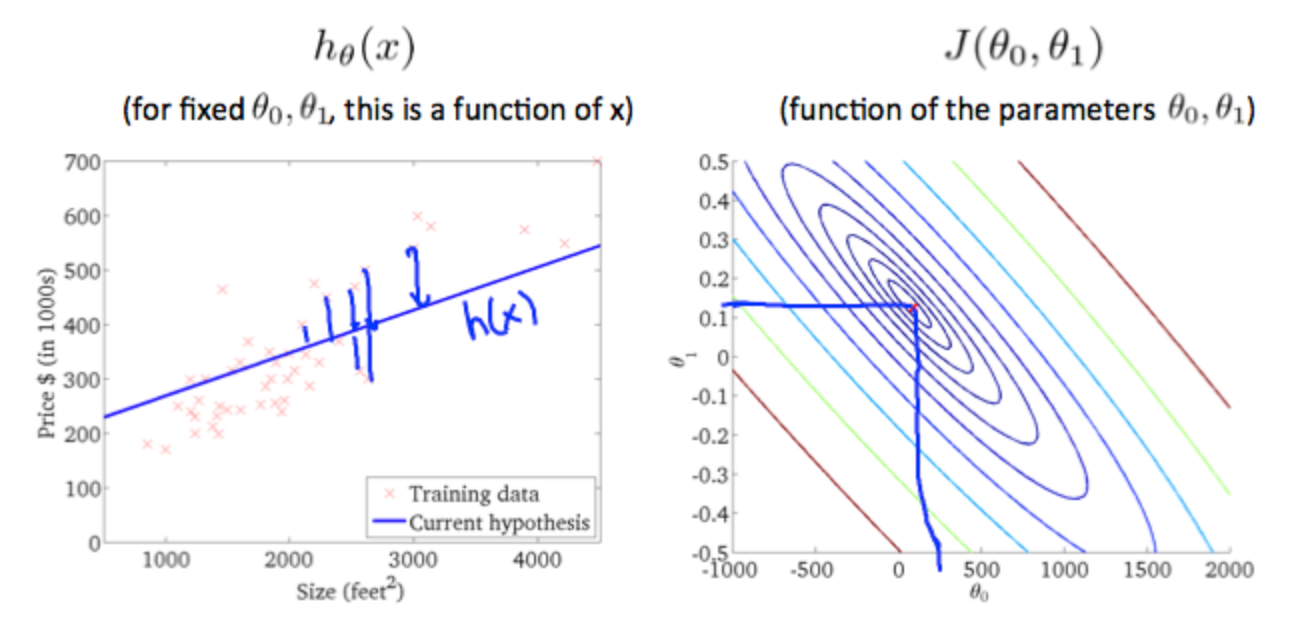
\includegraphics[width=0.6\textwidth]{figures/contour.png}
\end{figure}

\subsection{Parameter learning}

We want to estimate the parameters in the hypothesis function, which is where \textbf{gradient descent} comes in. Graphing our hypothesis function as a function of the parameter estimates gives a surface. Gradient descent uses the fact that the gradient is the direction towards the minimum (very roughly speaking) to perform an iterative movement towards the minimum. I would write more detail about gradient descent but I'm literally doing a summer project on optimisation so I don't think there's much point, refer to my optimisation notes for more details. This algorithm gives an iterate
\[\theta_j := \theta_j - \alpha \frac{\partial}{\partial \theta_j} J(\theta_0, \theta_1),\]
where $j=0,1$ represents the feature index number.
\begin{center}
    \textit{Update the parameters simultaneously, or else gradient descent won't work!}
\end{center}
(Note: this fact would be obvious if we employed the gradient operator $\nabla J(\theta_0, \theta_1)$ instead of Ng's notation, but I digress.)

When specially applied to linear regression, we can obtain a new form of gradient descent. Replacing the cost function and hypothesis function, we obtain the following iterate:
\begin{align*}
    \theta_0 &:= \theta_0 - \alpha \frac1m \sum_{i=1}^m (h_\theta(x_i) - y_i) \\
    \theta_1 &:= \theta_1 - \alpha \frac1m \sum_{i=1}^m ((h_\theta(x_i) - y_i)x_i)
\end{align*}
These can both be verified with some calculus.

\section{Week 2}

\subsection{Multivariate linear regression}

Linear regression with multiple variables is also known as \textbf{multivariate linear regression}. In the more general case, we can have the following:

\begin{center}
    \begin{tabular}{cl}
     $x_j^{(i)}$ & value of feature $j$ in the $i$th training example \\
     $x^{(i)}$ & the input of the $i$th training example \\
     $m$ & the number of training examples \\
     $n$ & the number of features
    \end{tabular}
\end{center}
The multivariate form of this is
\[h_\theta(x) = \theta_0 + \theta_1 x_1 + \theta_2 x_2 + \ldots + \theta_n x_n \quad \equiv \quad h_\theta(x) = \theta^\top x\]
where $\theta = \begin{pmatrix} \theta_0 & \theta_1 & \ldots & \theta_n \end{pmatrix}$ and $x = \begin{pmatrix} x_0 & x_1 & \ldots & x_n \end{pmatrix}^\top$.

For gradient descent in the multivariate case using Ng's notation we have the following iterate:
\[\theta_j := \theta_j - \alpha \frac1m \sum_{i=1}^m (h_\theta(x^{(i)}) - y^{(i)}) \cdot x_j^{(i)}, \quad \forall j \in \{0, \ldots, n\}.\]

We introduce a practical trick for gradient descent called \textbf{feature scaling}. The idea is to ensure that features are on a similar scale, making gradient descent faster. We get every feature into \textit{approximately} a $-1 \leq x_i \leq 1$ range. You can also perform \textbf{mean normalisation}, where we replace $x_i$ with $x_i - \mu_i$ to make features have approximately zero mean, making sure not to apply to $x_0 = 1$ or anything like that. You can also divide by the standard deviation $s_i$ instead of the range.

For gradient descent, we can also use something called the \textbf{automatic convergence test}. Declare convergence if $J(\theta)$ decreases by less than $\varepsilon$ in one iteration, where $\varepsilon$ is some small value. (It's difficult to choose this threshold value). If $\alpha$ is too small, we have a slow convergence rate, but if $\alpha$ is too large, we may not decrease on every iteration and thus may not converge.

We may also have a situation where we have polynomial regression. We can change the behaviour or curve of our hypothesis function by making it a quadratic, cubic or square root function (or any other form). For example, if our hypothesis function is $h_\theta(x) = \theta_0 + \theta_1 x$, we can create additional features based on $x_1$ to get a quadratic with $\theta_2 x_1^2$ or even a cubic with both $\theta_2 x_1^2$ and $\theta_3 x_1^3$ added.

\subsection{Computing parameters analytically}

We have been using iterative algorithms so far such as gradient descent, but for some problems we can solve for $\theta$ analytically. The \textbf{normal equation} formula (the Moore-Penrose pseudoinverse times $y$ for the enlightened) is the solution to the problem
\[\theta = (X^\top X)^{-1} X^\top y.\]
There is no need to do feature scaling or any other bollocks with the normal equation. However, the normal equation has complexity $\mathcal O(n^3)$ and you may need to compute the inverse of $X^\top X$, so it can be really slow for large $n$.

\begin{center}
\begin{tabular}{l|l}
Gradient Descent & Normal Equation \\
\hline
Need to choose $\alpha$ & No need to choose $\alpha$ \\
Needs many iterations & No need to iterate \\
$\mathcal O(kn^2)$ & $\mathcal O(n^3)$ and inverse \\
Works well when $n$ is large & Slow if $n$ is large
\end{tabular}
\end{center}

But look at the normal equation; we have an inverse. Not every matrix has an inverse. Using \texttt{pinv} in MATLAB gets around this in some fancy ways, but we should still be alarmed if $X^\top X$ is noninvertible, as there may be:
\begin{itemize}
    \item Redundant features, where two features are very closely related (linearly dependent)
    \item Too many features ($m \leq n$). In this case, delete some features or use ``regularisation''.
\end{itemize}

\section{Week 3}

\subsection{Classification and representation}

The problem of classifying a tumour as either malignant or benign. Assign 0 to benign and 1 to malignant. We can use a \textbf{threshold classifier}, which says
\[y = \begin{cases}
 1 & h_\theta(x) \geq 0.5 \\
 0 &  h_\theta(x) < 0.5.	
 \end{cases}
\]
But linear regression has some flaws. If we have some output way out of the linear regression line, the threshold classifier doesn't really work as it may misclassify based on the outlier. Linear regression to a dataset for classification is generally really bad. Another issue is that for linear regression, the hypothesis is not bounded to purely $\{0,1\}$.

In order to get around this, we develop a new technique called \textbf{logistic regression} (for purely historical reasons, it is considered regression, but it is really classification). We define the \textbf{sigmoid or logistic function}
\[g(z) = \frac{1}{1 + e^{-z}}, \quad h_\theta (x) = g(\theta^\top x) \quad \implies \quad h_\theta(x) = \frac{1}{1 + e^{-\theta^\top x}}\]
The sigmoid function appears as follows: 

\begin{figure}[H]
\centering	
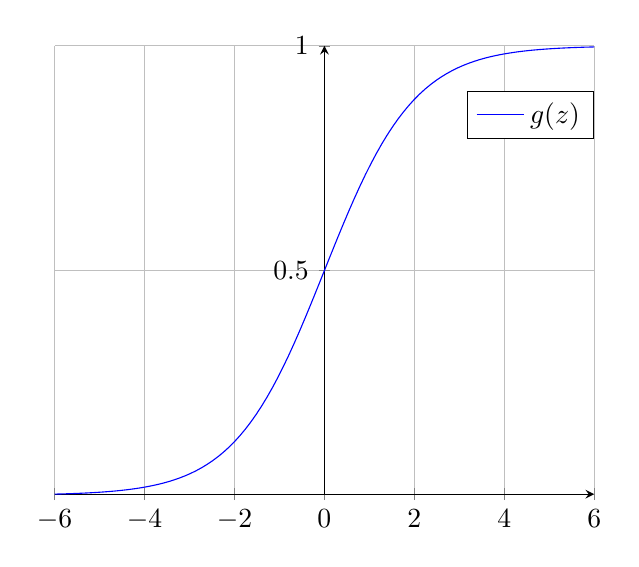
\begin{tikzpicture}[declare function={sigma(\x)=1/(1+exp(-\x));
sigmap(\x)=sigma(\x)*(1-sigma(\x));}]
\begin{axis}%
[
    grid=major,     
    xmin=-6,
    xmax=6,
    axis x line=bottom,
    ytick={0,.5,1},
    ymax=1,
    axis y line=middle,
    samples=100,
    domain=-6:6,
    legend style={at={(1,0.9)}}     
]
    \addplot[blue,mark=none]   (x,{sigma(x)});
    \legend{$g(z)$}
\end{axis}
\end{tikzpicture}
\end{figure}

We need to fit the parameters $\theta$ given a training set. We can interpret the hypothesis output as follows. $h_\theta(x)$ is the \textbf{estimated probability} that $y=1$ on input $x$. 

\begin{exmp}
	If $x = (x_0, x_1)^\top = (1, \text{tumor size})^\top$ and we obtain $h_\theta(x) = 0.7$, we can interpret that as the patient ``has a 70\% chance of the tumour being malignant''. We know that
	\begin{align*}
		\mathbb P(y = 0 \mid x; \theta) \mathbb P(y = 1 \mid x; \theta) &= 1 \\
		\mathbb P(y = 0 \mid x; \theta) &= 1 - \mathbb P(y = 1 \mid x; \theta)
	\end{align*}
	(I recognise that this probability stuff is a bit rough.)
\end{exmp}

For logistic regression, we can use the threshold to predict $y=1$ if $h_\theta(x) \geq 0.5$, and $y=0$ if $h_\theta(x) < 0.5$. This is equivalent to predicting $y=1$ if $\theta^\top x \geq 0$ and $y=0$ if $\theta^\top x < 0$. Suppose we have a training set which looks like the following, and that our hypothesis is
\[h_\theta(x) = g(\theta_0 + \theta_1 x_1 + \theta_2 x_2), \quad \theta = (-3, 1, 1)^\top.\]
Given this choice of hypothesis parameters, we predict $y=1$ if $-3 + x_1 + x_2 \geq 0$, and $y=0$ otherwise. The \textbf{decision boundary} is this function $-3 + x_1 + x_2$; it is the function that separates the area where $y=0$ and $y=1$. If the decision boundary is positive, we predict 1 and negative vice-versa.

We can also add higher-order terms to the features. For this decision boundary, we choose
\[h_\theta(x) = g(\theta_0 + \theta_1 x_1 + \theta_2 x_2 + \theta_3 x_1^2 + \theta_4 x^2_2), \quad \theta = (-1, 0, 0, 1, 1)^\top.\]
We predict $y=1$ if $-1 + x_1^2 + x_2^2 \geq 0$ (this is the equation of a circle when rearranging).

\begin{figure}[H]
	\centering
	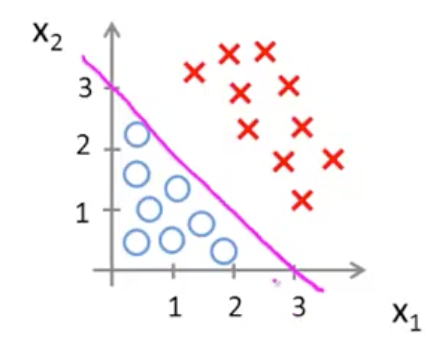
\includegraphics[height=10em]{figures/db1}
	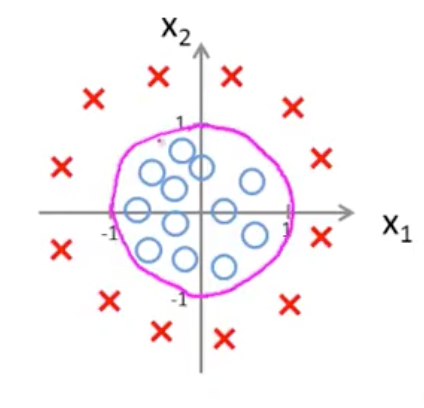
\includegraphics[height=10em]{figures/db2}
\end{figure}

\subsection{Logistic regression model}
Given the training set $\{(x^{(1)}, y^{(1)}), \ldots, (x^{(m)}, y^{(m)})\}$ of $m$ examples, with each example represented by a feature vector $x \in (x_0, x_1, \ldots, x_n)^\top (\mathbb R^{n+1}$, $x_0 = 1, y \in \{0,1\}$ and a hypothesis function $h_\theta(x) = \frac{1}{1 + e^{-\theta^\top x}}$, how do we choose parameters $\theta$?

Back in linear regression land, we formulated the cost function as
\[J(\theta) = \frac1m \sum_{i=1}^m \frac12 (h_\theta(x^{(i)} - y^{(i)})^2 = \frac1m \sum_{i=1}^m \mathrm{Cost}(h_\theta(x^{(i)}, y^{(i)}), \quad  \mathrm{Cost}(h_\theta(x^{(i)}, y^{(i)}) \triangleq \frac12 (h_\theta(x^{(i)}) - y^{(i)})^2.\]
This function worked fine for linear regression, but we are interested in logistic regression. This function is \textbf{nonconvex} for parameter $\theta$ in logistic regression, which means we can't run gradient descent and expect any sort of convergence.

Instead, we use the function
\[\mathrm{Cost}(h_\theta(x), y) = \begin{cases} -\log(h_\theta(x)) & y = 1 \\
 -\log(1 - h_\theta(x)) & y = 0	
 \end{cases}
\]

If our correct answer $y=0$, then the cost function will be 0 if our hypothesis function also outputs $0$. If our hypothesis approaches 1, then the cost function will tend to infinity. Conversely, if our correct answer $y=1$, then the cost function will be 0 if our hypothesis function outputs 1, and if our hypothesis approaches 0, then the cost function will tend to infinity. This function gives a convex and local-optima-free cost function $J(\theta)$.

We can actually rewrite this cost function more cleanly than before. Since $y=0$ or $1$ always, we can rewrite this function using a convex combination:
\[\mathrm{Cost}(h_\theta(x), y) = -y \log (h_\theta(x)) - (1 - y)\log(1 - h_\theta(x)).\]
We can fully write out our entire cost function as
\[J(\theta) = -\frac1m \sum_{i=1}^m \left( y^{(i)} \log(h_\theta(x^{(i)})) + (1 - y^{(i)}) \log(1 - h_\theta(x^{(i)}))\right)\]
or the equivalent vectorised
\[h = g(X\theta), \quad J(\theta) = \frac1m (-y^\top \log(h) - (1 - y)^\top log(1 - h)).\]
Gradient descent is also easy to implement; in fact, we obtain the exact same iterate
\[\theta_j := \theta_j - \frac{\alpha}{m} \sum_{i=1}^m (h_\theta(x^{(i)}) - y^{(i)}) x_j^{(i)} \quad  \equiv \quad \theta := \theta - \frac{\alpha}{m} X^\top (g(X\theta) - y).\]
Feature scaling also applies to gradient descent with logistic regression.

For optimisation problems, we also have more sophisticated algorithms such as conjugate gradient, BFGS and L-BFGS. They have a number of advantages, such as not needing to manually pick $\alpha$ and being faster than gradient descent, but this comes at the cost of being complicated (??). In MATLAB, use the \texttt{fminunc} function (minimise unconstrained).

\end{document}
